\begin{comment}
\end{comment}
\begin{frame}
\frametitle{Reference \hfill 
\includegraphics[height=0.5cm]{00_logo.png}}
\begin{columns}
  \column{0.1\textwidth}
  
  \column{0.6\textwidth}
	% \begin{enumerate}
	% 	\item 如果各个轴是正交的,那么很容易得到bias和scale:
	% \end{enumerate}
	[1] 贺一家,高翔 IMU传感器 \ 讲义.

	[2] A Robust and Easy to Implement Method for IMU Calibration without External Equipments.

	[3] An introduction to inertial navigation.

	...
  
  % \column{0.3\textwidth}
	% \begin{figure}[h]
	% 	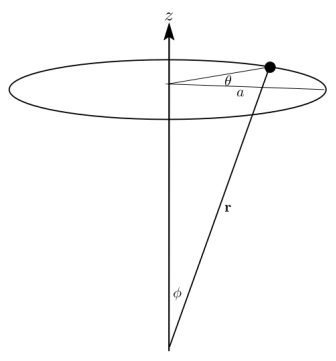
\includegraphics[trim=1.5 0 0 0, height=3.5cm,clip]{11_0.png}
	% 	% \caption{四个区域搜索空间}
  % \end{figure}
  
	\column{0.1\textwidth}

\end{columns}
\end{frame}

%%%%%%%%%%%%%%%%%%%%%%%%%%%%